\chapter{Misure di Resistenza ed Impedenza con DMM e LCR}
\label{chap:prima_prova}


\section*{Obiettivo}
\label{sec:ob_first}

L'obiettivo primario di questa iniziale esperienza di laboratorio consiste nell'acquisire familiarità con l'utilizzo di strumentazione di base per le misurazioni, con le corrette procedure di misurazione e con la valutazione dell'incertezza associata, nel caso di misurazioni di resistenza e impedenza.
\newline \newline
A tale scopo ci è stato dato un resistore dal valore nominale di 1,5 $\Omega$ (valore nominale apprezzabile ad occhio nudo, tramite la visualizzazione delle lineette di colore marrone, verde, oro (vedi figura \ref{fig:resistore})) con un incertezza del 5\% (dato che l'ultimo anello è di colore oro).

\begin{figure}[h]
    \centering
    \includegraphics[height=10cm]{resistoretab.png}
    \caption{Tabella che raffigura il codice dei colori di un resistore}
    \label{fig:resistore}
\end{figure}
\FloatBarrier











\section{Misure di resistenze con multimetro portatile}
\label{sec:mult_port}

\begin{figure}[h]
    \centering
    \includegraphics[height=10cm]{multimetro_port.png}
    \caption{Multimetro utilizzato (Hewlett Packard 974A)}
    \label{fig:multimetro_port}
\end{figure}
\FloatBarrier

Il multimetro HP 974A è dotato di un display a 4 ½ cifre, il quale rappresenta uno strumento con 4 cifre principali e un'ulteriore cifra riservata per indicare il segno e, eventualmente, il valore della cifra più significativa della misurazione. Per calcolare la resistenza con un valore nominale dichiarato dal produttore pari a (1500 ± 7,5) m$\Omega$, abbiamo utilizzato il pulsante "RANGE" per impostare il valore di fondo scala, ovvero il limite superiore che il multimetro può "misurare", a 500 $\Omega$. Dato che lo strumento ha un campo di misura pari a 1/50000 del valore di fondo scala, il passo di quantizzazione, indicato come "Q", è pari a
\begin{equation}
    Q = \frac{V_{F_S}}{50000} = \frac{500}{50000} = 10 m\Omega
\end{equation}
con un incertezza di quantizzazione pari a: 
\begin{equation}
    U_q = \frac{Q}{2} = 5 m\Omega
\end{equation}

Procediamo con la valutazione dell'incertezza di \textbf{tipo B}, basata sull'utilizzo di informazioni note a priori quali le specifiche metrologiche degli strumenti adoperati. L’incertezza del dispositivo è data da una formula binomia composta da una parte proporzionale alla lettura e da un’altra pari a un numero fisso di LSB, quindi 
 proporzionale alla portata. Le specifiche del costruttore dello strumento, per misure di resistenze, sono le seguenti:

\begin{figure}[h]
    \centering
    \includegraphics[height=4cm]{incertezza_port.png}
    \caption{Specifice di incertezza dello strumento utilizzato (Hewlett Packard 974A)}
    \label{fig:Incertezza_multimetro_port}
\end{figure}
\FloatBarrier

Avendo impostato un valore di fondo scala pari a 500 $\Omega$ possiamo notare dalla precedente tabella un’incertezza pari a ±(0,06\% + 2) $\Omega$ , dove il primo termine è proporzionale alla lettura e il secondo alla portata. Si noti che per misure di ampiezza è possibile definire un modello semplificato di uno strumento per misure statiche, del tipo:

\begin{figure}[h]
    \centering
    \includegraphics[height=3cm]{modello_semplificato.png}
    \label{fig:modello}
\end{figure}
\FloatBarrier

Su cui definiamo un errore totale sulla misura del tipo:

\begin{equation}
    E_t(x) = \Delta Gx + O + inl(x) + e_q(g(x)) + N
\end{equation}

%\begin{figure} [h]
%    \centering
%    \includegraphics[height=2cm]{errore_port.png}
%    \label{fig:errore port}
%\end{figure}

Attraverso una serie di passaggi otteniamo l'incertezza come:
\begin{equation}
    |E_t| \equiv |y_q - x| \equiv | \Delta G_x + O + inl(x) + e_q(g(x)) | \leq 
\end{equation}
applichiamo una disuguaglianza triangolare
\begin{equation*}
    \leq | \Delta Gx | + | O | + | inl(x) | + | e_q(g(x)) | \leq 
\end{equation*}
applichiamo una disuguaglianza errore-incertezza
\begin{equation*}
    \leq U_G|x| + U_o + U_{inl} + U_q \cong U_G|y_q| + U_o + U_{inl} +U_q \equiv U_{tot}
\end{equation*}

Dove, ipotizzando di unire l'incertezza di non linearità integrale nell'incertezza di portata, posso scrivere $U_g$ (incertezza di guadagno), $U_o$ (incertezza di portata dell'offset) e $U_q$ (incertezza di quantizzazione) come: 
\begin{equation}
\left\{\begin{array}{l}
    | \Delta G \cdot y_q | \leq U_G |y_q| \ , \ con \ U_g=0,06\% \\
| O + inl(x) + e_q(g(x)) | \leq U_{o+inl+q} \ , \ con \ U_{o+inl+q}=2LSB
\end{array}\right.
\end{equation}

Quindi, chiamando Q, passo di quantizzazione e $V_L$ valore letto (supponiamo di usare il primo valore letto nella tabella \label{mult_port}):

\begin{equation*}
\begin{array}{l}
U(R) \equiv U_G \cdot V_L + U_{o+inl+q} \cdot Q \equiv 0,06\% \cdot 1,62\Omega + 2 \cdot 0,01 \Omega \\ \\
\equiv (0,972 + 20) m\Omega \equiv 0,03 \Omega
\end{array}
\end{equation*}

sapendo che possiamo esprimere la resistenza misurata $R_M$ e il range della resistenza r(R) come:
\begin{equation*}
    R_M \equiv(1,62 \pm 0,03) \Omega
\end{equation*}
\begin{equation*}
    r(R) \equiv [1,59 \Omega \div 1,65 \Omega]
\end{equation*}

Va notato che l'inclusione dell'errore di non linearit\'a integrale nel secondo termine dell'incertezza fornita dal produttore ( proporzionale alla portata) rende tale termine non solamente un errore di offset puro, ma include anche l'errore di quantizzazione. Pertanto, nel caso di differenze tra misurazioni, non possiamo semplicemente sottrarre l'errore di offset.
Notiamo, usando la resistenza nominale di $(1500 \pm 7,5) m\Omega$ e graficandola con la (2.9) che i due range di valori non sono compatibili.

\begin{figure}[h]
    \centering
    \includegraphics[height=4cm]{range.png}
    \caption{Differenza dei due range}
    \label{fig:range}
\end{figure}
\FloatBarrier

Effettivamente, la misura eseguita utilizzando il multimetro portatile fornisce una stima non corretta poiché include errori casuali a causa della singola misurazione anziché una media di più valori letti. Inoltre, lo strumento non consente la compensazione degli errori sistematici poiché non dispone di funzioni di calibrazione. Infine, non si è tenuto conto degli errori dovuti alle resistenze di contatto tra i cavi, i puntali e il resistore. Il contributo di tutti questi effetti influisce sul risultato finale della misura.

Se vogliamo quantificare l'accuratezza della misura, assumiamo come valore "vero" della grandezza misurata il valore nominale della resistenza. Facendo questa assunzione, possiamo ottenere una stima dell'errore sistematico come differenza tra il risultato della misura e il valore nominale del componente misurato:
\begin{equation}
    E_S \equiv 1,62 - 1,50 = 0,12\Omega
\end{equation}
L’accuratezza relativa “a” di una misura può essere espressa in funzione di tale errore 
stimato in errore relativo mediante la seguente espressione: 
\begin{equation}
     a \equiv 1 - \left| \frac{E_S}{R_{NOMINALE}}\right| \equiv 92\%
\end{equation}


\subsection*{La nostra prova}
\label{sub:nosta_prova_first}


\vspace{0.5cm}
%\begin{wrapfigure}{l}{0.3\textwidth}
\FloatBarrier
\begin{figure}[h]
    \centering
    \includegraphics[width=5cm]{Gameboy_62.jpg}
    \label{fig:mult_port_nostro}
\end{figure}
\FloatBarrier
%\end{wrapfigure}
    

Quando usiamo il multimetro portatile abbiamo disposto i puntali in maniera pi\'u stabile possibile, applicando una buona pressione per ottenere una misurazione pi\'u fedele possibile,
Abbiamo fatto 10 ripetizioni in modo da ricavare l'incertezza totale, con il contributo valutato di tipo B relativamente alla specifica di strumento utilizzato.

\begin{table}[!ht]
    \centering
    \begin{tabular}{|c|c|c|c|}
    \hline
        \textbf{R}$\bm{[\Omega]}$ & \textbf{Q}$\bm{[\Omega]}$ & \textbf{Uq} $\bm{[\Omega]}$ & $\bm{U_r}$ \\ \hline
        1,62 & 1,00E-02 & 5,00E-03 & 2,10E-02 \\ \hline
        1,61 & 1,00E-02 & 5,00E-03 & 2,10E-02 \\ \hline
        1,61 & 1,00E-02 & 5,00E-03 & 2,10E-02 \\ \hline
        1,62 & 1,00E-02 & 5,00E-03 & 2,10E-02 \\ \hline
        1,60 & 1,00E-02 & 5,00E-03 & 2,10E-02 \\ \hline
        1,60 & 1,00E-02 & 5,00E-03 & 2,10E-02 \\ \hline
        1,62 & 1,00E-02 & 5,00E-03 & 2,10E-02 \\ \hline
        1,61 & 1,00E-02 & 5,00E-03 & 2,10E-02 \\ \hline
        1,60 & 1,00E-02 & 5,00E-03 & 2,10E-02 \\ \hline
        1,61 & 1,00E-02 & 5,00E-03 & 2,10E-02 \\ \hline
    \end{tabular}
    \caption{Multimetro portatile 974A, fondo scala di 500 $\Omega$}
    \label{tab:mult_port}
\end{table}
\FloatBarrier

\vspace{4cm}
%---------Multimetro da Banco---------%
\section{Misure di resistenza con multimetro da banco}
\label{sec:mult}


\begin{figure}[h]
    \centering
    \includegraphics[height=5cm]{mult_banco.png}
    \caption{Multimetro HP Hewlett Packard 34401A}
    \label{fig:mult_banco}
\end{figure}
\FloatBarrier

Il multimetro HP34401A possiede un display a 6 ½ cifre. 
Per il calcolo della resistenza di valore nominale pari a (1500 ± 7,5) m$\Omega$, impostiamo la portata dello strumento a 100,0000 $\Omega$, lo strumento a 6 ½ cifre ha un campo di misura 
pari a 1/1000000 del valore di fondo scala e quindi il passo di quantizzazione Q sar\'a: 
\begin{equation}
    Q \equiv \frac{V_{FS}}{CM} \equiv \frac{10^2}{10^6} = 0,0001 \Omega
\end{equation}
Con l'incertezza di quantizzazione $U_q$ pari a:
\begin{equation}
    U_q \equiv \frac{Q}{CM} \equiv 0,00005 \Omega
\end{equation}

Quando abbiamo lavorato con il multimetro da banco, abbiamo dapprima lavorato in modalità "2 terminali" (attivata premendo la modalità "$\Omega$", e poi "2W" che ci permette di lavorare a due morsetti).

\begin{figure}[h]
    \centering
    \includegraphics[height=2cm]{mult_banco_zoom.png}
    \caption{Zoom sui tasti premuti}
    \label{fig:mult_banco_zoom}
\end{figure}
\FloatBarrier

Come prima operazione abbiamo cortocircuitato i morsetti, premendo il tasto null, in modo che il valore di resistenza interna del conduttore dei cavi venga preso in considerazione permettendoci di tarare lo strumento, mostrando una misurazione prossima a zero (nel nostro caso abbiamo visualizzato a display, impostato a 6 cifre e mezzo, il valore 0,000134).

% L HO RIMOSSA MOMENTANEAMENTE PERCHE' NON MI PIACE LA IN MEZZO TROPPO BIANCO
%\begin{figure}[h]
%    \centering
%    \includegraphics[height=4cm]{2Morsetti_432.jpg}
%    \label{fig:2morsetti}
%\end{figure}
%\FloatBarrier

\'E importante notare che se la resistenza dei cavi è comparabile o superiore alla resistenza che si desidera misurare, il risultato della misura potrebbe essere influenzato significativamente dal contributo della resistenza dei cavi, dunque per ridurre gli errori sistematici:
\begin{equation}
    Risultato = Valore \ \ letto - Valore\ \ NULL
\end{equation}

\begin{figure}[h]
    \centering
    \includegraphics[height=9cm]{tabella_mult_banco.png}
    \label{fig:tab_mult_banco}
\end{figure}
\FloatBarrier

Avendo impostato un valore di fondo scala pari a 100,0000 $\Omega$, in un ambiente con una temperatura pari a (23 $\pm$ 5)°C, facciamo riferimento all'incertezza $\pm$(0,010 $\% \pm 0,004 \%$), con il primo termine proporzionale alla lettura e il secondo proporzionale alla portata.
Ragionando come prima, ipotizzando di unire l'incertezza di non linearità integrale nell'incertezza di portata, posso scrivere $U_g$ (incertezza di guadagno), $U_o$ (incertezza di portata dell'offset) e $U_q$ (incertezza di quantizzazione) come: 
\begin{equation}
\left\{\begin{array}{l}
| \Delta G \cdot y_q | \leq U_G |y_q| \ , \ con U_g=0,01\% \\ 
| O + inl(x) + e_q(g(x)) | \leq U_{o+inl+q} \ , con \ U_{o+inl+q}=0,004\%
\end{array}\right.
\end{equation}
Quindi, chiamando P, portata e $V_L$ valore letto (supponiamo di usare il primo valore letto nella tabella \label{mult_port}):
\begin{equation*}
    U(R) \equiv U_G \cdot V_L + U_{o+inl+q} \cdot P \equiv 0,01\% \cdot 1,648\Omega + 0,004 \% \cdot 100 \Omega \equiv 0,004 \Omega 
\end{equation*}

dove U(R) è stato arrotondato per difetto.

\begin{table}[!ht]
\resizebox{\textwidth}{!}{%
    \centering
    \begin{tabular}{|c|c|c|c|c|c|c|}
    \hline
        \textbf{V misurata [V]} & \textbf{V di Cortocircuito [V]} & \textbf{V [V]} & \textbf{Fondo scala} $\bm{[\Omega]}$ & \textbf{Q} $\bm{[\Omega]}$ & $\bm{U_q\ \ [\Omega]}$ & $\bm{U_V}$ \textbf{[V]} \\ \hline
        1,648 & 0,133 & 1,515 & 100 & 0,0001 & 0,00005 & 0,0041515 \\ \hline
        1,614 & 0,133 & 1,481 & 100 & 0,0001 & 0,00005 & 0,0041481 \\ \hline
        1,627 & 0,133 & 1,494 & 100 & 0,0001 & 0,00005 & 0,0041494 \\ \hline
        1,614 & 0,133 & 1,481 & 100 & 0,0001 & 0,00005 & 0,0041481 \\ \hline
        1,432 & 0,133 & 1,299 & 100 & 0,0001 & 0,00005 & 0,0041299 \\ \hline
        1,466 & 0,133 & 1,333 & 100 & 0,0001 & 0,00005 & 0,0041333 \\ \hline
        1,441 & 0,133 & 1,308 & 100 & 0,0001 & 0,00005 & 0,0041308 \\ \hline
        1,468 & 0,133 & 1,335 & 100 & 0,0001 & 0,00005 & 0,0041335 \\ \hline
        1,475 & 0,133 & 1,342 & 100 & 0,0001 & 0,00005 & 0,0041342 \\ \hline
        1,493 & 0,133 & 1,36 & 100 & 0,0001 & 0,00005 & 0,004136 \\ \hline
    \end{tabular}%
    }
    \caption{Multimetro 34401A (6$\sfrac{1}{2}$ cifre), 2 Morsetti}
    \label{tab:mult_2w}
\end{table}
\FloatBarrier

 Sapendo che la resistenza misurata col multimetro è 1,648 $\Omega$, il risultato della misura si esprime come R=(+1,648 $\pm$ 0,005)$\Omega$, abbiamo operato anche con un sistema a quattro morsetti(metodo Kelvin)


\begin{figure}[h]
    \centering
    \includegraphics[height=5cm]{quattro_morsetti.png}
    \caption{Metodo Kelvin a 4 morsetti}
    \label{fig:quattro morsetti}
\end{figure}





Successivamente, sempre con lo stesso multimetro da banco, abbiamo lavorato in modalità "4 terminali" (attivata sempre premendo la modalità "$\Omega$", e poi successivamente "4W" per lavorare a quattro morsetti).

\begin{wrapfigure}{l}{0.3\textwidth}
    \centering
    \includegraphics[width=0.28\textwidth]{4Morsetti_472.jpg}
    \label{fig:4morsetti}
\end{wrapfigure}
Anche in questo caso abbiamo nuovamente cortocircuitato i morsetti, premendo nuovamente il tasto null per tarare lo strumento e riavere un valore associato al cortocircuito pi\'u prossimo allo zero possibile in presenza del cortocircuito (nel nostro caso 0,004).


Attraverso la prima coppia di morsetti (Hi, Lo), lo strumento inietta la corrente nota come "$I_0$" nella resistenza. Questa corrente attraversa le boccole (Hi, Lo) dove si incontra con la resistenza di contatto, che può falsare la misura standard a due fili (impostando $\Omega$2W sul pannello frontale del multimetro).

Per evitare questo problema, tramite l'altra coppia di morsetti di sensing (Hi, Lo), viene prelevata la tensione su due punti più vicini al resistore. Utilizzando questa configurazione (impostando $\Omega$4W sul pannello frontale del multimetro), le cadute di tensione sulle resistenze di contatto presenti sulle boccole che portano la corrente al resistore in prova possono essere escluse dalla tensione da misurare, garantendo una misurazione più accurata.

Si effettua l'operazione di NULL in modo analogo al caso precedente, misurando un valore di resistenza pari a R = 1,478 $\Delta$. Dalla teoria, questo valore dovrebbe essere più accurato rispetto al caso del multimetro a due morsetti. Utilizzando il modello precedente per il calcolo dell'incertezza, otteniamo:

\begin{equation}
    \left\{\begin{array}{l}
| \Delta G \cdot y_q | \leq U_G |y_q|,    con U_g=0,01\%
\\ | O + inl(x) + e_q(g(x)) | \leq U_{o+inl+q}, con U_{o+inl+q}=0,004\%
\end{array}\right.
\end{equation}


    


Quindi, chiamando P, portata e $V_L$ valore letto (supponiamo di usare il primo valore letto nella tabella \label{mult_port}):

\begin{equation*}
    U(R) \equiv U_G \cdot V_L + U_{o+inl+q} \cdot P \equiv 0,01\% \cdot 1,478\Omega + 0,004 \% \cdot 100 \Omega \equiv 0,004 \Omega 
\end{equation*}
(dove il risultato è stato arrotondato per difetto)
Notiamo che l’incertezza in questo caso non è cambiata, con R=(+1,478 $\pm$ 0,005)$\Omega$



\begin{table}[!ht]
\resizebox{\textwidth}{!}{%
    \centering
    \begin{tabular}{|c|c|c|c|c|c|c|}
    \hline
        \textbf{V misurata [V]} & \textbf{V di Cortocircuito [V]} & \textbf{V [V]} & \textbf{Fondo scala} $\bm{[\Omega]}$ & \textbf{Q} $\bm{[\Omega]}$ & $\bm{U_q\ \ [\Omega]}$ & $\bm{U_V}$ \textbf{[V]} \\ \hline
        1,478 & 0,004 & 1,474 & 100 & 0,0001 & 0,00005 & 0,0041474 \\ \hline
        1,478 & 0,004 & 1,474 & 100 & 0,0001 & 0,00005 & 0,0041474 \\ \hline
        1,478 & 0,004 & 1,474 & 100 & 0,0001 & 0,00005 & 0,0041474 \\ \hline
        1,478 & 0,004 & 1,474 & 100 & 0,0001 & 0,00005 & 0,0041474 \\ \hline
        1,478 & 0,004 & 1,474 & 100 & 0,0001 & 0,00005 & 0,0041474 \\ \hline
        1,478 & 0,004 & 1,474 & 100 & 0,0001 & 0,00005 & 0,0041474 \\ \hline
        1,478 & 0,004 & 1,474 & 100 & 0,0001 & 0,00005 & 0,0041474 \\ \hline
        1,478 & 0,004 & 1,474 & 100 & 0,0001 & 0,00005 & 0,0041474 \\ \hline
        1,478 & 0,004 & 1,474 & 100 & 0,0001 & 0,00005 & 0,0041474 \\ \hline
        1,478 & 0,004 & 1,474 & 100 & 0,0001 & 0,00005 & 0,0041474 \\ \hline
    \end{tabular}%
    }
    \caption{Multimetro 34401A (6$\sfrac{1}{2}$ cifre), 4 Morsetti}
    \label{tab:mult_4w}
\end{table}
\FloatBarrier



Osserviamo questa volta che utilizzando il multimetro da banco a 6 ½ cifre si ottiene una stima più precisa del valore misurato rispetto all'utilizzo del multimetro portatile descritto precedentemente. Questi miglioramenti possono essere attribuiti alla capacità dello strumento da banco di ridurre gli errori sistematici mediante l'implementazione di funzioni adeguate.

Il multimetro da banco a 6 ½ cifre offre una maggiore precisione grazie alla sua elevata risoluzione e alla possibilità di compensare gli errori sistematici tramite funzioni avanzate di calibrazione e correzione. Ciò consente di ottenere misurazioni più accurate e affidabili, riducendo l'effetto degli errori di offset, delle non linearità e di altri fattori che potrebbero influenzare la precisione della misura.

Inoltre, lo strumento da banco può offrire un controllo più preciso delle condizioni operative, come la compensazione della resistenza dei cavi o la selezione della modalità di misura più adatta alle specifiche dell'applicazione. Ciò contribuisce ulteriormente a migliorare l'accuratezza complessiva della misurazione.

In conclusione, usando una resistenza con valore nominale di (1500 ± 7,5) m$\Omega$, con il multimetro da banco otteniamo una stima pari a R=(+1,648 $\pm$ 0,005)$\Omega$ per la misurazione a due morsetti, mente otteniamo una stima pari a R=(+1,478 $\pm$ 0,005)$\Omega$ per la misurazione a 4 morsetti.

\begin{figure}[h]
    \centering
    \includegraphics[height=3cm]{banco_misure.png}
    \label{fig:range}
\end{figure}

eeeeeeeeeeeeeeeeeeeeeeeeeeeeeeeeeeeeeeeeeee doveva uscire che i 4w stava dentro il range del resistore, non so se dovremmo commentare o no la cosaaaaaaaaaaaaaaaaaaaaaaaaaaaaaaaaaaaaa
\newline
Volendo quantificare gli errori sistematici:
\begin{equation}
    E_S(2W) \equiv 1,648 - 1,500 = 0,148 \Omega
\end{equation}
\begin{equation}
    | E_S(4W) | \equiv | 1,478 - 1,500  |= 0,022 \Omega
\end{equation}
che portano alle seguenti accuratezze: 
\begin{equation}
    a_{(2W)} \equiv 1 - \left| \frac{E_{S(2W)}}{R_{NOMINALE}} \right| \equiv 91\%
\end{equation}
\begin{equation}
    a_{(4W)} \equiv 1 - \left| \frac{E_{S(4W)}}{R_{NOMINALE}} \right| \equiv 91\%
\end{equation}

AIUTOOOOOOOOOOOOOOO dovrebbero essere percentuali pi§ alte del multimetro da banco














%----------LCR-----------%
\section{Misure con LCR-Meter}
\label{sec:lcr}

\subsection{Strumentazione}
\label{sub:strum}
Lo scopo dell’esercitazione è quello di effettuare misure di impedenze per mezzo 
dell’LCR-meter e di valutare l’incertezza di tali misure facendo uso delle specifiche 
del costruttore, cioè eseguendo valutazioni dell’incertezza di tipo B.
Il disegno illustrativo del montaggio dell’apparecchiature è il seguente:

\begin{figure}[h]
    \centering
    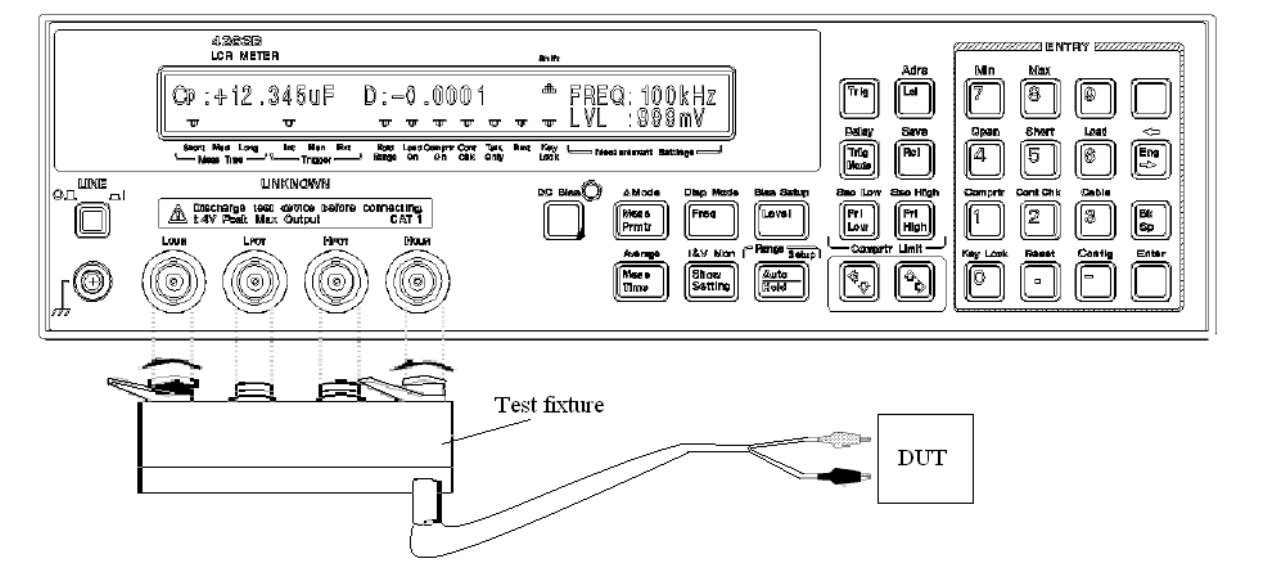
\includegraphics[height=6cm]{media/LCR_meter.png}
    \label{fig:LCR_meter}
\end{figure}
\FloatBarrier

\begin{itemize}
    \item AGILENT LCR-meter 4263B;
    \item Kelvin clip leads di lunghezza pari a 1m;
    \item Test fixture;
    \item Resistenza con valore nominale pari a $(1000\pm50)m\Omega$;
    \item Capacità con valore nominale pari a $(6800\pm340)pF$;
\end{itemize}


I seguenti strumenti consentono di determinare i parametri di induttanza, capacità, resistenza, fattore di merito e coefficiente di perdita per induttori, condensatori e resistori, utilizzando gli schemi equivalenti prefissati degli oggetti sottoposti ad analisi.

L'oggetto in prova viene sottoposto a basse tensioni e correnti durante il test, con un livello di segnale che può essere regolato dall'operatore da alcuni millivolt a 1 volt efficace, quando si lavora a tensione fissa.

Il tempo trascorso tra l'inizio di una misura e l'inizio della successiva è di circa qualche decina di millisecondi e varia in base all'incertezza richiesta. Più piccola è l'incertezza richiesta, maggiore sarà il tempo necessario per la misurazione. Un esempio di valore possibile è 25 ms (short).

L'esercitazione è iniziata reimpostando il dispositivo ai suoi valori predefiniti e collegando il supporto di test al pannello frontale come illustrato nello schema di montaggio.

L'esercitazione è iniziata con il ripristino dei valori predefiniti del dispositivo e il collegamento del supporto di test al pannello frontale come mostrato nello schema di montaggio. Successivamente, possiamo procedere con la calibrazione dello strumento al fine di ridurre al minimo gli errori sistemici che possono influire sulle misurazioni.

Per evitare gli errori di sfasamento causati dalla lunghezza del cavo, abbiamo impostato la lunghezza del cavo a un metro utilizzando il comando corrispondente nel pannello frontale dell'LCR.

\begin{figure}[ht]
    \centering
    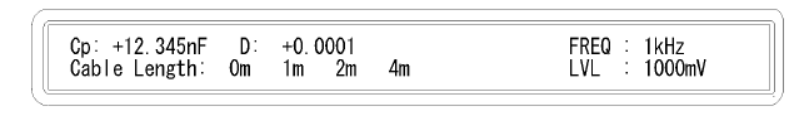
\includegraphics[height=2cm]{media/pannello_frontale_LCR.png}
    \caption{Pannello Frontale LCR}
    \label{fig:pannello_frontale_LCR}
\end{figure}
\FloatBarrier

Successivamente, abbiamo proceduto con la correzione OPEN/SHORT dello strumento impostando la frequenza massima dell'LCR. A questa frequenza, eventuali variazioni delle condizioni operative dello strumento, come temperatura e umidità, potrebbero influire negativamente sull'incertezza della misura.



\subsection{Impedenze}
\label{sub:z}

Tramite l'LCR-Meter abbiamo svolto l'ultima parte della nostra prima esperienza.

Di solito, per effettuare misurazioni di impedenza, è necessario stabilire un piano di riferimento sull'ingresso del DUT (Device Under Test) nel pannello frontale. L'LCR ci permette di fare ciò fissando la lunghezza del cavo utilizzato. Tuttavia, è importante cercare di eliminare le impedenze residue causate dalla presenza del Test Fixture nel pannello frontale dello strumento.

Innanzitutto abbiamo calibrato lo strumento per compensare gli errori sistematici introdotti dallo strumento stesso, dando come riferimento due carichi noti (il circuito virtualmente chiuso e aperto), premendo sul tassto blu dello strumento e aspettando la dicitura "short correction complete".
Per fare la prova, abbiamo avuto la possibilità di impostare vari valori di frequenza a partire da 100Hz, abbiamo impostato un tempo di misura medio ??? e impostato il modello capacità ideale con collegamento parallelo (premendo in successione i tasti CP-D e CP-RP).
Partiamo con i 100Hz, e misuriamo la resistenza (R) e reattanza (X, nel nostro caso leggermente negativà perché prevale l'effetto induttivo). Abbiamo fatto così per ogni valore della frequenza presente nella seguente tabella.  


\begin{table}[!ht]
\centering
\begin{tabular}{|c|c|c|}
\hline
\textit{\textbf{Frequenza}} \textbf{[Hz]} & \textbf{R [$\bm{\Omega}$]}  & \textbf{X [m$\bm{\Omega}$]}  \\ \hline
100Hz                       & 1,4630    & -0,04      \\ \hline
120Hz                       & 1,4628    & -0,05      \\ \hline
1kHz                        & 1,4625    & -0,52      \\ \hline
10kHz                       & 1,4622    & -5,12      \\ \hline
100kHz                      & 1,4635    & -51,50     \\ \hline
\end{tabular}
\caption{LCR, misura Impedenza, Tempo di misura: Long}
\label{tab:lcr_z}
\end{table}
\FloatBarrier


Se rappresentiamo le precedenti misure in modulo e fase avremo i seguenti grafici:
%Mancano i due grafici relativi a questa tabella%
%\begin{figure}[ht]
%    \centering
%    \includegraphics[height=2cm]{media/grafico_modulo.png}
%    \caption{Grafico del modulo}
%    \label{fig:grafico_modulo}
%\end{figure}
%
%\begin{figure}[ht]
%    \centering
%    \includegraphics[height=2cm]{media/grafico_fase.png}
%    \caption{Grafico della fase}
%    \label{fig:grafico_fase}
%\end{figure}

Dai grafici precedenti si può notare che alle alte frequenze è necessario considerare gli effetti parassiti della resistenza reale, che tendono ad aumentare il valore nominale della resistenza linearmente con la frequenza.

Il circuito equivalente prevede un'induttanza in serie alla resistenza e una capacità in parallelo alla serie RL. I valori delle impedenze parassite dipendono dalla tecnica di costruzione.

Alle basse frequenze, l'effetto della capacità e dell'induttanza può essere trascurato in quanto la capacità si comporta come un circuito aperto e l'induttanza come un cortocircuito. Aumentando la frequenza, la capacità tende ad abbassare il valore della resistenza, mentre l'induttore tende ad aumentarlo fino a quando, alla frequenza $1/2\pi\sqrt{LC}$, la coppia LC entra in risonanza compensandosi reciprocamente.

Per il calcolo dell'incertezza delle misure di resistenza e reattanza riportate nella tabella precedente, dobbiamo fare riferimento alle specifiche del costruttore. Per il calcolo dell'incertezza, è necessario applicare la seguente formula:

\begin{equation}
    A_e = A + \frac{BCZ_S}{|Z_X|} + \frac{D}{|Z_X|} + \frac{|Z_X|}{E} \hspace{0,8cm} con \hspace{0,2cm} |Z_X| \leq 100\Omega
\end{equation}

dove $Z_X$ è il valore misurato dell’impedenza Z. L’incertezza di $|Z|$ è uguale a quella di 
R e di X per cui, consultando le tabelle di incertezza fornite dal costruttore, avremo:


%TABELLA INCERTEZZA IMPEDENZA%
\begin{table}[!ht]
\centering
\begin{tabular}{|c|c|c|c|c|c|c|c|}
\hline
\textbf{A}      & \textbf{B}      & \textbf{C} & \textbf{D [$\bm{\Omega}$]} & \textbf{E [$\bm{\Omega}$]}  & $\bm{Z_s \ \ [\Omega]}$ & $\bm{Z_x \ \ [\Omega]}$ & $\bm{U_z}$ \textbf{(Ae)} \\ \hline
0,005  & 0,0009 & 1 & 0,01      & 2,80E+08  & 1          & 1,4630     & 0,0125  \\ \hline
0,005  & 0,0009 & 1 & 0,01      & 2,80E+08  & 1          & 1,4628     & 0,0125  \\ \hline
0,004  & 0,0003 & 1 & 0,0165    & 2,80E+07  & 1          & 1,4625     & 0,0155  \\ \hline
0,004  & 0,0003 & 1 & 0,075     & 2,80E+06  & 1          & 1,4622     & 0,0555  \\ \hline
0,0097 & 0,0011 & 1 & 0,75      & 2,80E+05  & 1          & 1,4635     & 0,5229  \\ \hline
\end{tabular}
\caption{Tabella di incertezza fornita dal costruttore, con $U_z$ l'incertezza}
\label{tab:lcr_z_sheet}
\end{table}
\FloatBarrier

Con l'incertezza di quantizzazione $U_q$ pari a:
\begin{equation}
    U_q = \frac{Q}{CM} = 0,00005 \Omega
\end{equation}



%-------------Capacità----------- %
\subsection{Capacità}
\label{sub:c}
Come ultima parte della prova abbiamo misurato la capacità del condensatore.
Premiamo in successione "CP" (capacità), "RP" (resistenza parallela) e poi "D" (per il valore della tangente dell'angolo di perdita). Questa procedura è stata ripetuta per tutti i valori di frequenza (partendo da 100kHz, arrivando fino ai 100Hz).


\begin{table}[ht]
\centering
\resizebox{\textwidth}{!}{%
\begin{tabular}{|c|c|c|c|}
\hline
\rowcolor[HTML]{CFE2F3} 
\textit{Frequenza} {[}Hz{]} & Cp {[F]} & Rp {[}$\Omega${]} & D  \\ \hline
100Hz                       & 6,98E-09    & 1,27E+08     & 0,0018     \\ \hline
120Hz                       & 6,88E-09    & 1,33E+08     & 0,0017      \\ \hline
1kHz                        & 6,96E-09    & 5,42E+06     & 0,0039      \\ \hline
10kHz                       & 6,89E-09    & 2,60E+05     & 0,0095      \\ \hline
100kHz                      & 6,70E-09    & 1,87E+04     & 0,0147      \\ \hline
\end{tabular}%
}
\caption{LCR, misura della capacità}
\label{tab:lcr_c}
\end{table}
\FloatBarrier

Per il calcolo dell’incertezza dobbiamo applicare le seguenti formule:

\begin{equation}
\begin{split}
        A_e = A + \frac{BCZ_X}{|Z_S|} + \frac{D}{|Z_X|} + \frac{|Z_X|}{E} \hspace{0,8cm} con \hspace{0,2cm} |Z_X| > 100\Omega \\
        A_e = A + \frac{BCZ_S}{|Z_X|} + \frac{D}{|Z_X|} + \frac{|Z_X|}{E} \hspace{0,8cm} con \hspace{0,2cm} |Z_X| \leq 100\Omega
\end{split}
\end{equation}

dove $|Z_X|$ è il valore dell'impedenza Z ottenuta convertendo il valore della capacità parallelo (Cp) per mezzo del seguente diagramma di conversione:

\begin{figure}[H]
    \centering
    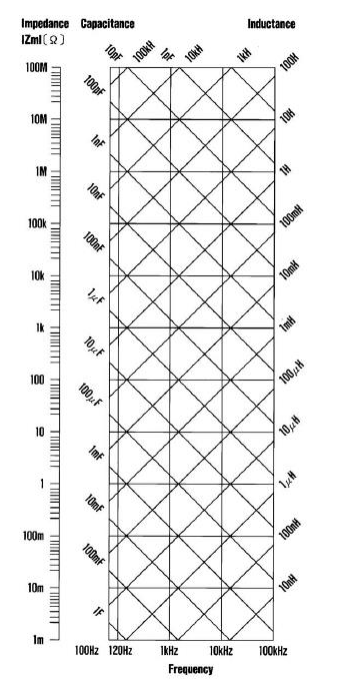
\includegraphics{media/diagramma_conversione_Cp.png}
    \caption{Diagramma di conversione}
    \label{fig:diag_conv_Cp}
\end{figure}
\FloatBarrier

Consultando le tabelle di incertezza fornite dal costruttore avremo:

\begin{table}[H]
\centering
\resizebox{\textwidth}{!}{%
\begin{tabular}{|c|c|c|c|c|c|c|c|}
\hline
\rowcolor[HTML]{CFE2F3} 
A      & B      & C & D {[}$\Omega${]} & E {[}$\Omega${]} & Zs {[}$\Omega${]} & Zx {\tiny(Cp convertito)}  {[}$\Omega${]} & Uz (Ae) \\ \hline
0,0048  & 0,00055 & 1 & 0,01      & 2,80E+08  & 100000          & 228054,8849     & 0,0069  \\ \hline
0,0048  & 0,00055 & 1 & 0,01      & 2,80E+08  & 100000          & 192858,9781     & 0,0065  \\ \hline
0,0011  & 0,0002 & 1 & 0,0165    & 2,80E+07  & 10000          & 22880,2391     & 0,0024  \\ \hline
0,0016  & 0,0002 & 1 & 0,075     & 2,80E+06  & 1000          & 2311,4843     & 0,0029  \\ \hline
0,0112 & 0,0011 & 1 & 0,75      & 2,80E+05  & 100          & 237,4632     & 0,0178  \\ \hline
\end{tabular}%
}
\caption{Tabella di incertezza fornita dal costruttore, con Uz l'incertezza}
\label{tab:lcr_c_sheet}
\end{table}
\FloatBarrier

L’incertezza della resistenza parallelo, invece, si calcola come:

\begin{equation}
        U_{R_P} = \pm \frac{RP_X \times D_e}{D_X \mp D_e}  \\
\end{equation}

dove $RP_X$ indica il valore misurato della resistenza parallelo in $\Omega$, $D_e$ è l’incertezza di 
$D$, mentre $D_X$ è il valore misurato di $D$.

L’incertezza dell’angolo di perdita, $D_e$, si calcola come:

\begin{equation}
    D_e = \pm \frac{A_e}{100}
\end{equation}

Se il valore misurato di $D$ risulta ad essere maggiore di 0,1 , allora bisogna 
moltiplicare $D_e$ per $(1+D_X)$. L’incertezza sulla resistenza parallelo si applica solo 
quando il valore misurato di $D$ è minore di 0,1.

Nella seguente tabella è riassunto quanto detto precedentemente:

\begin{table}[H]
\centering
\resizebox{\textwidth}{!}{%
\begin{tabular}{|c|c|c|c|}
\hline
\rowcolor[HTML]{CFE2F3} 
RPx {[$\Omega$]} & De  & Dx  & U(Rp) \\ \hline
1,27E+08                    & 0,00006868827448    & 0,0018     & 5,06E+06    \\ \hline
1,33E+08                    & 0,00006549558296    & 0,0017    & 5,32E+06      \\ \hline
5,42E+06                    & 0,00002375477324    & 0,0039     & 3,32E+04      \\ \hline
2,60E+05                    & 0,00002920273675    & 0,0095     & 8,00E+02      \\ \hline
1,87E+04                    & 0,0001781856214    & 0,0147     & 2,29E+02      \\ \hline
\end{tabular}%
}
\caption{LCR, misura della resistenza}
\label{tab:lcr_c_RPx}
\end{table}
\FloatBarrier


